%%%%%%%%%%%%%%%%%%%%%%%%%%%%%%%%%%%%%%%%%
% Short Sectioned Assignment
% LaTeX Template
% Version 1.0 (5/5/12)
%
% This template has been downloaded from:
% http://www.LaTeXTemplates.com
%
% Original author:
% Frits Wenneker (http://www.howtotex.com)
%
% License:
% CC BY-NC-SA 3.0 (http://creativecommons.org/licenses/by-nc-sa/3.0/)
%
%%%%%%%%%%%%%%%%%%%%%%%%%%%%%%%%%%%%%%%%%

%----------------------------------------------------------------------------------------
%	PACKAGES AND OTHER DOCUMENT CONFIGURATIONS
%----------------------------------------------------------------------------------------

\documentclass[paper=a4, fontsize=11pt]{scrartcl} % A4 paper and 11pt font size

\usepackage[T1]{fontenc} % Use 8-bit encoding that has 256 glyphs
\usepackage{fourier} % Use the Adobe Utopia font for the document - comment this line to return to the LaTeX default
\usepackage[english]{babel} % English language/hyphenation
\usepackage{amsmath,amsfonts,amsthm} % Math packages
\usepackage{graphicx}
\usepackage{caption}
\usepackage{subcaption}

\usepackage{lipsum} % Used for inserting dummy 'Lorem ipsum' text into the template

\usepackage{sectsty} % Allows customizing section commands
\allsectionsfont{\centering \normalfont\scshape} % Make all sections centered, the default font and small caps

\usepackage{fancyhdr} % Custom headers and footers
\pagestyle{fancyplain} % Makes all pages in the document conform to the custom headers and footers
\fancyhead{} % No page header - if you want one, create it in the same way as the footers below
\fancyfoot[L]{} % Empty left footer
\fancyfoot[C]{} % Empty center footer
\fancyfoot[R]{\thepage} % Page numbering for right footer
\renewcommand{\headrulewidth}{0pt} % Remove header underlines
\renewcommand{\footrulewidth}{0pt} % Remove footer underlines
\setlength{\headheight}{13.6pt} % Customize the height of the header

\numberwithin{equation}{section} % Number equations within sections (i.e. 1.1, 1.2, 2.1, 2.2 instead of 1, 2, 3, 4)
\numberwithin{figure}{section} % Number figures within sections (i.e. 1.1, 1.2, 2.1, 2.2 instead of 1, 2, 3, 4)
\numberwithin{table}{section} % Number tables within sections (i.e. 1.1, 1.2, 2.1, 2.2 instead of 1, 2, 3, 4)

% \setlength\parindent{0pt} % Removes all indentation from paragraphs - comment this line for an assignment with lots of text

%----------------------------------------------------------------------------------------
%	TITLE SECTION
%----------------------------------------------------------------------------------------

\newcommand{\horrule}[1]{\rule{\linewidth}{#1}} % Create horizontal rule command with 1 argument of height

\title{	
\normalfont \normalsize 
\textsc{Imperial College London} \\ [20pt] % Your university, school and/or department name(s)
% \horrule{0.5pt} \\[0.4cm] % Thin top horizontal rule
\huge Advanced Computer Architecture Coursework One Report \\ % The assignment title
% \horrule{2pt} \\[0.5cm] % Thick bottom horizontal rule
}

\author{Richard Evans\\ rce10@ic.ac.uk} % Your name

\date{\normalsize\today} % Today's date or a custom date

\begin{document}

\maketitle % Print the title

\section{Microarchitecture issues in Local Assembly using the Finite Element Method for a Helmholtz problem}

\subsection{Introduction to the problem}

The purpose of this coursewok was to study the effect of various architectural features on the performance of the provided Helmholtz benchmark using SimpleScalar Simplesim and the SimpleScalar implementation of the HelmHoltz application given.

Inspection of the HelmHoltz disassembly shows the main body of execution is concerned with alternation between arithmetic operations, multiplies and load/stores.

\subsection{Simple Analysis of RUU (Register Update Unit) Size}

\subsubsection{Measure of IPC (Instructions Per Cycle)}

To begin, I varied the size of the RUU using the basic bash script varyarch provided with the coursework.  The value of RUU size was varied from 2 to 256 and the IPC (Instructions Per Cycle) of the execution of the code recorded into a data file.  This data was then plotted onto a graph using gnuplot.  The graph of results can be seen in figure 1.1.a.

\begin{figure}
\centering
\begin{subfigure}{0.5\textwidth}
  \centering
   \includegraphics[width=\linewidth]{graphs/ruuipc.eps}
  \caption{IPC of System}
\end{subfigure}%
\begin{subfigure}{0.5\textwidth}
  \centering
   \includegraphics[width=\linewidth]{graphs/ruuenergy.eps}
  \caption{Energy Consumption of System}
\end{subfigure}
\caption{Variance in RUU Size}
\end{figure}

It can be seen from this figure that a very small RUU size causes incredibly poor performance of the architecture when running the HelmHoltz code.  The register update unit is responsible for the control over interleaved instruction pipelines and controls where an instruction is issued and when, along with register renaming.  If the RUU size is small, for example 2 in the simplescalar architecture under test, only two instructions can ever be in flight at a time.  As a result these instructions can only be replaced as they finish, causing a cripplingly slow execution time, ~0.4IPC reported by SimpleSim. This is largely because the constant need for load store instructions complete incredibly slowly (relatively speaking) and so execution is bottlenecked by this.  Incresing RUU size means more instructions can be in flight at a time and so theoretically should increase system performance.  It can be seen, however, that performance of the system peaks with an RUU size of 16 with an IPC of ~1.5.  This performance then drops very slightly to ~1.45 and plateaus.  This is because other components of the architecture are causing a bottleneck to the system and limiting the rate at which execution can occur.

\subsubsection{Measure of Energy Usage}

Having investigated the performance implications of varying the RUU size I then looked at the energy consumption of the system as a whole using the varyarch-energy script provided which runs using SimpleSim-wattch which also calculated energy usage information.  As with varyarch, the size of the RUU was varied from 2 to 256, the results of which where then also plotted using gnuplot and can be seen in figure 1.1.b.

It can be seen from this figure that the energy usage of the architecture is at a minimum with an RUU of size 16.  This is because it is the mimumum required size to provide optimum performance given the other architectural features of the system.  An increase of RUU beyond 16 causes the RUU to occupy more `silicon', and so use more power, without the runtime of the program decreasing, hence causing a higher total use of power.

\subsection{Finding the System Bottleneck}

Having identified that the performance of the system can be optimised by increasing the RUU size to 64 from its default of 16 (which it has already been shown is optimal for the default configuration of other parameters).  Since 64 should theoretically allow greater performance, I then proceeded to vary other parameters of the system, with RUU size held at 64, to find which of the other architecture parameters was the bottleneck, causing the plateau in system performance.

I wrote several more scripts in the style of varyarch which set the RUU size to 64 and varied another parameter, writing the results into a data log.  These results were then graphed using gnuplot until I found the culprit parameter which increased the IPC most: LSQ (Load Store Queue) size.  Having seen that increasing LSQ size allowed the largest increase in IPC of the system, I wrote a new script which would vary RUU size and LSQ size incrementally. These results were then plotted in a heatmap, shown in figure 1.2.a.

This figure shows that as LSQ size and RUU size increase together, so does the performance of the architecture when running the HelmHoltz code.  This can be explained by the high number of Load/Store instructions in the disaasembly of the code and the relative slow execution time of these instructions.

Having plotted the performance with variance in RUU and LSQ size as a heatmap, I then did the same for energy consumption of the system, as shown in figure 1.2.b.

\begin{figure}
\centering
\begin{subfigure}{0.5\textwidth}
  \centering
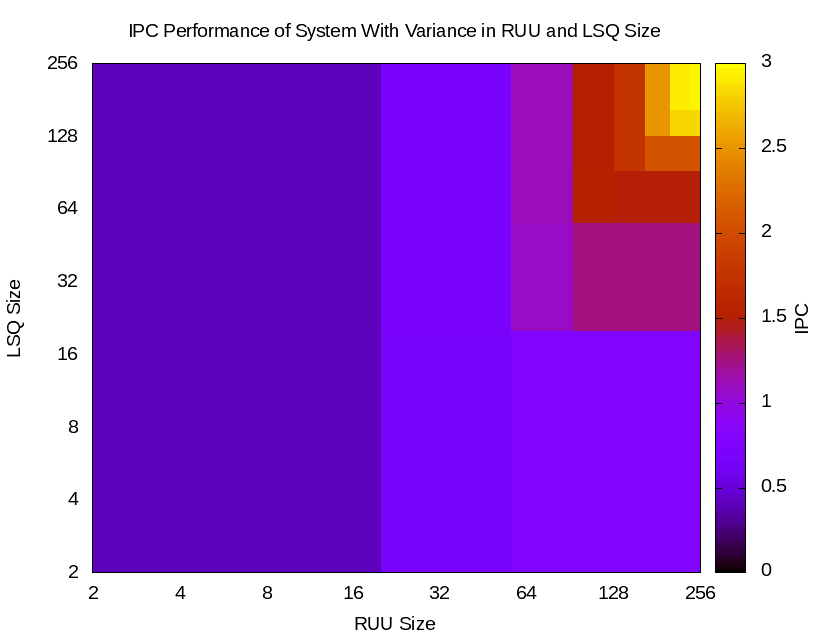
\includegraphics[width=\linewidth]{graphs/ruulsqipc.png}
 \caption{IPC Measurement}
\end{subfigure}%
\begin{subfigure}{0.5\textwidth}
  \centering
  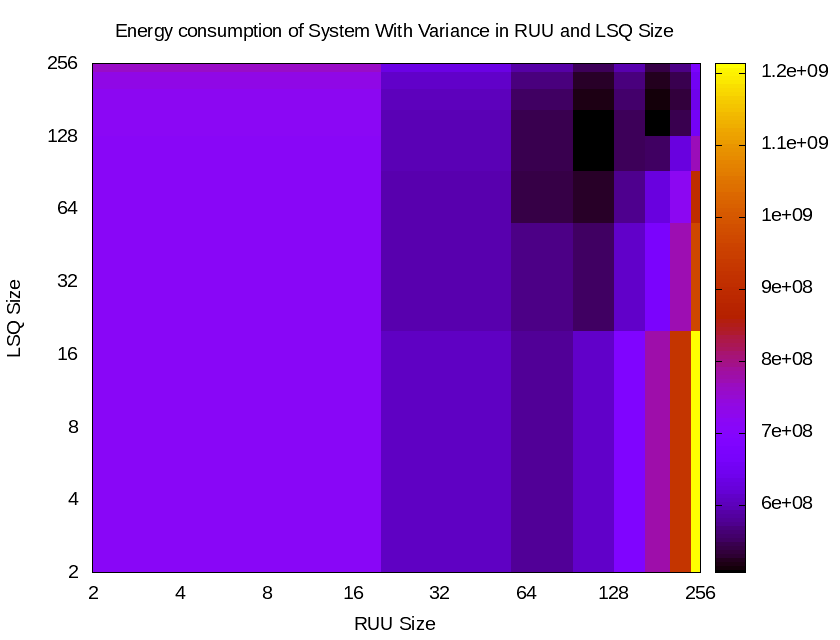
\includegraphics[width=\linewidth]{graphs/ruulsqenergy.png}
 \caption{Energy Measurement}
\end{subfigure}
\caption{Variances in IPC and energy with RUU and LSQ Size}
\end{figure}

It can be seen from this figure that whilst IPC increases consistently with increase in both RUU and LSQ size to a maxima with both set to 256, that this is not actually the most power efficient pair of values for the execution of the system.  This is actually found with both set to 128.  This is because the increase in IPC does not outweigh the extra cost of powering the silicon required.

\subsection{Finding the Energy Efficient `Sweet Spot'}

For the final part of the coursework we were to try and find the energy efficient `sweet spot' of architecture configuration which would use the least energy to execute the HelmHoltz code.  I interpreted this question to mean; ``find the configuration of the architecture parameters which allows completion of the HelmHoltz code with minimum total energy used, even at the expense of IPC and so total execution time''.

To find the mimumum power efficiency I considered the different aspects of the system and how SimpleSim calculates power consumption of the system.  I was using the powermeasurement for cc1, which assumes that each unit is is fully on if any of its ports are accessed in that cycle.

It therefore made sense to me that reducing the amount of complexity of the architecture and minimising active functional units would reduce the measured power consumed.  I wrote multiple scripts to find the optimal power consumption for each parameter as varied, and combined these  results and identified parameters into one configuration.

My final `optimal' configuration flags for the SimpleScalar system are: \\
-issue:width 1 -commit:width 1 -fetch:ifqsize 1 -decode:width 1 -res:ialu 1 -res:imult 1 \\ -res:fpalu 1 -res:fpmult 1 -bpred nottaken -issue:inorder true -issue:wrongpath false \\ -ruu:size 4 -lsq:size 4

\begin{figure}
\centering
 \makebox[\textwidth]{\includegraphics[width=0.68\paperwidth]{graphs/energyuse.eps}}
 \caption{Energy performance with variance in RUU and LSQ size}
\end{figure}

The energy used with this configuration is shown in comparison to the energy consumption of the default configuration in figure 1.3.  Whilst this implementation is very simple and does provide a very low total power consumption, it is very naive and simple, and with an IPC of only 0.606, executes very slowly.  In industry, an engineer would likely use a better metric to make design decisions, for example taking total power divided by cycles per instruction, as this would lead a design to be penalised by low execution, encouraging a better balance of power consumed and execution time.

\end{document}